\documentclass{article}
\usepackage{graphicx,amsmath,amsfonts,amsthm,physics,tikz} % Required for inserting images
\usepackage{hyperref}
\usepackage[colorinlistoftodos]{todonotes}
\usepackage{xcolor}
\usepackage{listings}
%\usepackage{minted}
\usepackage[normalem]{ulem}

\usepackage{pgfplots,pgf-pie, multirow}
\pgfplotsset{compat=1.18}
\setlength{\tabcolsep}{10pt}
\setlength{\arrayrulewidth}{0.6pt}
\renewcommand{\arraystretch}{1.175}

% \setlength{\parskip}{5pt}
\begin{document}
    \title{Gel Filtration Chromatography}
    \author{Sabarno Saha}
    \date{\today}
    \maketitle
    \section{Aim}
        Determination of Column Dead Volume using Gel Filtration Chromatography
        \section{Principle}
        The seperation between different molecules is done on the basis of molecule size and shape. This experiment is done in a cylindrical column with a stationary phase 
        which are beads made up of pores that span the long column kept in a mobile phase or buffer. Smaller molecules spend a larger time inside the beads than the larger molecules and 
        thus, the smaller molecules elute later(after a larger volume of the mobile phase has passed through).
        \section{Materials Used}
        \begin{enumerate}
            \item Sephadex G-75 as the packing material
            \item Blue Dextran as the dye to measure the column void volume
            \item NaCl Buffer
            \item Micropipettes
            \item Spectrophotometer
            \item 1.5 ml tubes
        \end{enumerate}
        \section{Procedure}
        \begin{enumerate}
            \item The column was given to us filled with \textbf{Sephadex G-75} as the stationary phase material and NaCl as the buffer solution which was our mobile phase
            \item Around 2\% of the bed volume, Blue dextran was measured, added and mixed with the buffer.
            \item The preparation was then poured into the column.
            \item And then buffer was added continuously to put pressure on the Blue Dextran Molecules.
            \item The buffer was also added as so as to prevent the column from running dry.
            \item The buffer was drained out onto another tube and was done so till the Blue Dextran Started pouring out.
            \item Then on the first appearance of the Blue Dextran molecules, they were poured onto 1.5 ml tubes.
            \item Then the tubes were filled with 500 $\mu$l buffer.
            \item The stopcock was closed after all the Blue Dextran had passe through it.
            \item The absorbance of every sample was recorded at 610 wavelength. The sample with the maximum absorbance was noted.
            \item The volume of the buffer collected in the 15mL tube was later added to the volume of the Blue Dextran collected till the maximum absorbance.The total is the dead volume
                $V_0$ of the tube.
        \end{enumerate}
        \section{Results}
    \begin{table}[!h]
    \centering
        
        \begin{tabular}{|p{0.50\textwidth}|p{0.50\textwidth}|}
        \hline 
        Sample & Absorbance Value \\
            \hline 
            1 & 0.630 \\ 
            \hline 
            2 & 1.076 \\
            \hline 
            3 & 0.991 \\
            \hline 
            4 & 0.694 \\
            \hline 
            5 & 0.181 \\
                \hline
        \end{tabular}
    \end{table}
    % \setlength{\parindent}{5pt}

    \begin{figure}
        \centering
        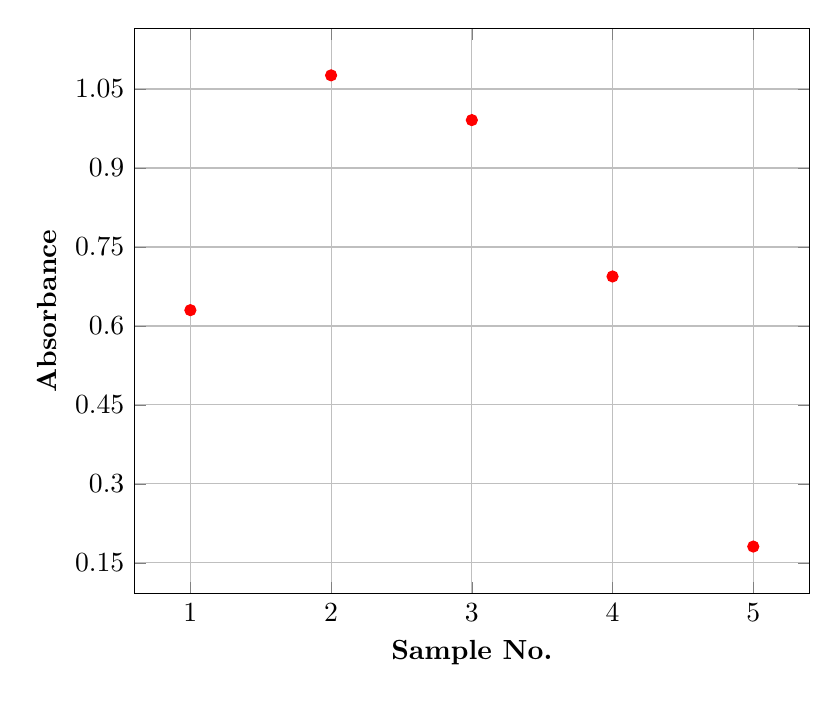
\begin{tikzpicture}
            \begin{axis}[
            width =4 in,
                xlabel=\textbf{Sample No.},
                ylabel=\textbf{Absorbance},
                grid=major,
                xtick={1,2,3,4,5,6},
                ytick={0, 0.15, 0.3, 0.45, 0.6, 0.75, 0.9, 1.05, 1.2}]
            \addplot[only marks,color=red,mark=*] coordinates {
                (1,0.630)
                (2,1.076)
                (3,0.991)
                (4,0.694)
                (5,0.181)
               };
            \end{axis}
        \end{tikzpicture}
        \caption{Absorbance of each sample}
    \end{figure}
    \newpage
    \subsection{Column Data}
    \begin{itemize}
        \item Bed Volume = 22.4 ml
        \item Amount of Blue Dextran Added over the volume = 448 $\mu$L
        \item Amount of buffer collected in the 15mL tube = 7mL
        \item Amount of Blue Dextran till the maximum absorbance = 1 mL
    \end{itemize}
    \section{Conclusion}
    We conclude that the total void volume for the column and stationary phase is around 8mL(7mL+1mL).
\end{document}

